\documentclass[
  usenames,svgnames, %xcolor options
  compress,
  %handout,
  ]{beamer}

\mode<presentation> {
  \usetheme{Singapore}
  \useinnertheme[shadow]{rounded}
  \usefonttheme[onlymath]{serif}
  \setbeamertemplate{navigation symbols}{\insertframenumber{}/\inserttotalframenumber}
}

\usepackage{xspace}
\newcommand{\TheProject}{\texttt{OpenDreamKit}\xspace}

\usepackage{hyperref}
\usepackage{listings} % For typesetting source code (verbatim, etc.)
\usepackage{graphicx}
\usepackage{tikz}

\usepackage{xcolor}
\definecolor{blue}{rgb}{0.2,0.2,0.7} 
\def\blue{\color{blue}}
\def\green{\color{green}}
\def\red{\color{red}}
\def\purple{\color{purple}}
\def\gray{\color{gray}}
\def\grey{\color{gray}}

% \guillemotleft and \guillemotright or just use >> or <<.
\usepackage[T1]{fontenc}
\usepackage[utf8]{inputenc}
\usepackage{xspace}

%% Sage
\newcommand{\SAGEp}{Sage}
\newcommand{\SAGE}{Sage\xspace}
\newcommand{\SAGEplus}{\SAGEp$^{++}$}
\newcommand{\Sage}{\texttt{Sage}\xspace}
\newcommand{\mupad}{\texttt{MuPAD}\xspace}
\newcommand{\maple}{\texttt{Maple}\xspace}
\newcommand{\magma}{\texttt{Magma}\xspace}
\newcommand{\python}{\texttt{Python}\xspace}
\newcommand{\cython}{\texttt{Cython}\xspace}
\newcommand{\mathematica}{\texttt{Mathematica}\xspace}
\newcommand{\starcombinat}{\texttt{$\ast$-Combinat}\xspace}
\newcommand{\mupadcombinat}{\texttt{MuPAD-Combinat}\xspace}
\newcommand{\sagecombinat}{\texttt{Sage-Combinat}\xspace}

\colorlet{structure}{red!65!black}

\title{{\huge \color{red} OpenDreamKit}\\
  Open Digital Research Environment Toolkit\\
  for the Advancement of Mathematics\\}

\subtitle{A personal perspective}


\begin{document}

\author{Nicolas M. Thiéry}
\begin{frame}
  \maketitle

  \Huge
  \centerline{\url{OpenDreamKit.org}}
\end{frame}

\begin{frame}{For me, it all started there}
  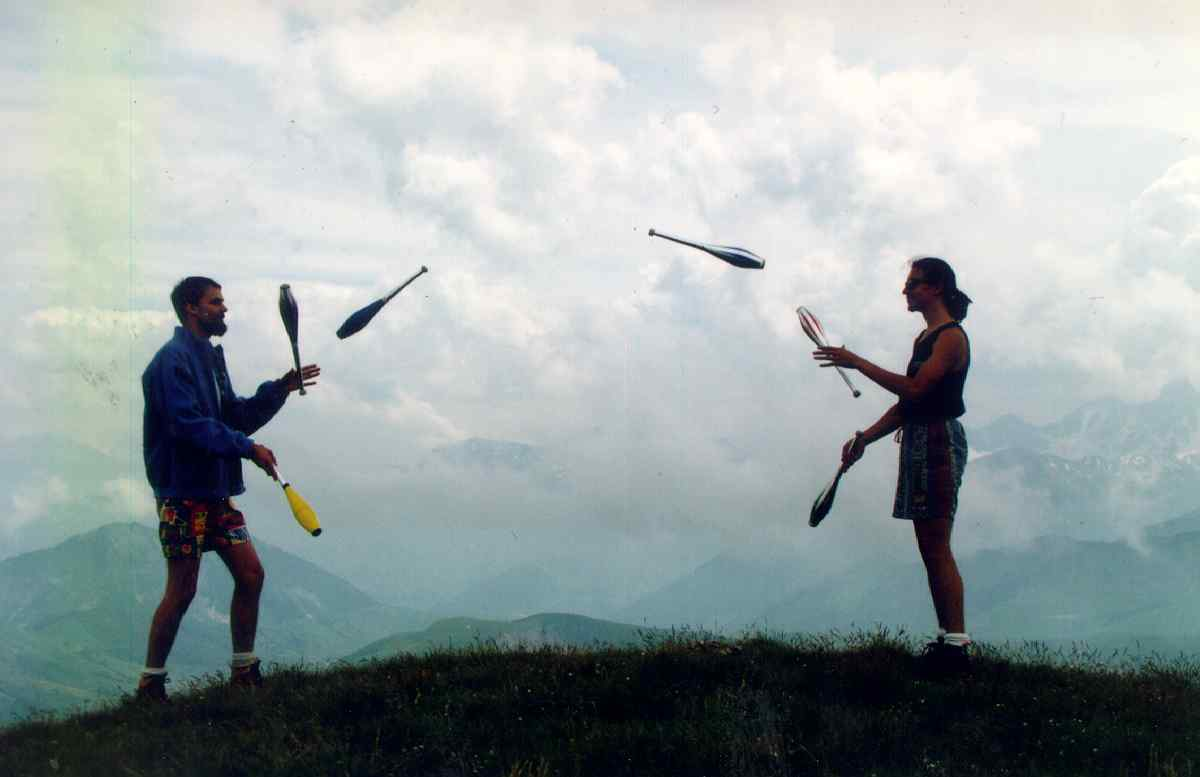
\includegraphics[width=\textwidth]{Pictures/haut2.jpg}
\end{frame}

% - Since 20 years, I am doing research in algebraic combinatorics. And
%   like about everybody here, computer exploration is a fundamental tool.
%
% - I am also am a big fan of free software, both from the ethics and practical
%   points of view
%
% - From the beginning a big fan of software packages like GAP, Singular, Pari
%   demonstrated that, with a few dedicated leaders, whole communities
%   of researchers could get together, and share their work, and build
%   the tools they need.

% - I wanted the same in my community. One constraint is that we
%   need a platform that integrates together tools from many different
%   areas of maths. So I ended up being a happy Sage developer.

% - For a long time, to keep being happy, I strived hard to not
%   depend on funding so that I could focus on coding and community
%   building.  But with time it became tricky.

\begin{frame}{For me, it all started there}

  \begin{block}{A question of Bruce Westbury at FPSAC 2013}
    Given unlimited funding, what would you do with it for Sage?
  \end{block}

\end{frame}

\begin{frame}{Context}
  \begin{block}{Emergence in the last decade(s) of a vibrant ecosystem
      of open source software for pure mathematics}

    \begin{itemize}
    \item Specialized libraries: GAP, Linbox, PARI/GP, MPIR, Singular,
      ...
    \item General purpose systems: Sage, ...
    \item Online databases: LMFDB, ...
    \item Interactive computing environments:\\
      IPython/Jupyter, SageMathCloud, ...
    \item Together with the wider Scientific Python ecosystem
    \end{itemize}
  \end{block}
  \pause
  \bigskip

  \begin{block}{Viable open source alternatives to Maple, Mathematica,
      Matlab, Magma, ...}
    \begin{itemize}
    \item Research
    \item Education
    \item Industry?
    \end{itemize}
  \end{block}
\end{frame}


\begin{frame}
  \begin{block}{A successful development model ...}
    \begin{itemize}
    \item By users, for users
    \item Indirect funding via research grants
    \item Large international developer communities (300 for Sage)
    \end{itemize}
  \end{block}
  \pause

  \begin{block}{... with some limitations}
    \begin{itemize}
    \item Some highly technical tasks are lagging behind:
      \begin{itemize}
      \item Hard to justify work on them for a researcher
      \item Hard to justify work on them on a research grant
      \end{itemize}
    \item Impeding the wide adoption of those systems
    \item Impeding collaborations between systems
    \end{itemize}
  \end{block}
  \pause

  \begin{block}{A need for funding for:}
    \begin{itemize}
    \item A couple full time developers
    \item Community building
    \end{itemize}
  \end{block}
\end{frame}

\begin{frame}{An opportunity suggested by Eugenia, January 2014}

  \begin{block}{Virtual Research Environments}
    A call of the H2020 European Research Infrastructures Work Programme
  \end{block}
  \pause

  \begin{block}{Definition}
    Groups of researchers, typically widely dispersed who are working
    together through ubiquitous, trusted and easy access to services
    for scientific data, computing and networking, in a
    \emph{collaborative virtual environment}.
  \end{block}
\end{frame}

\begin{frame}{Virtual Research Environments in Math}
  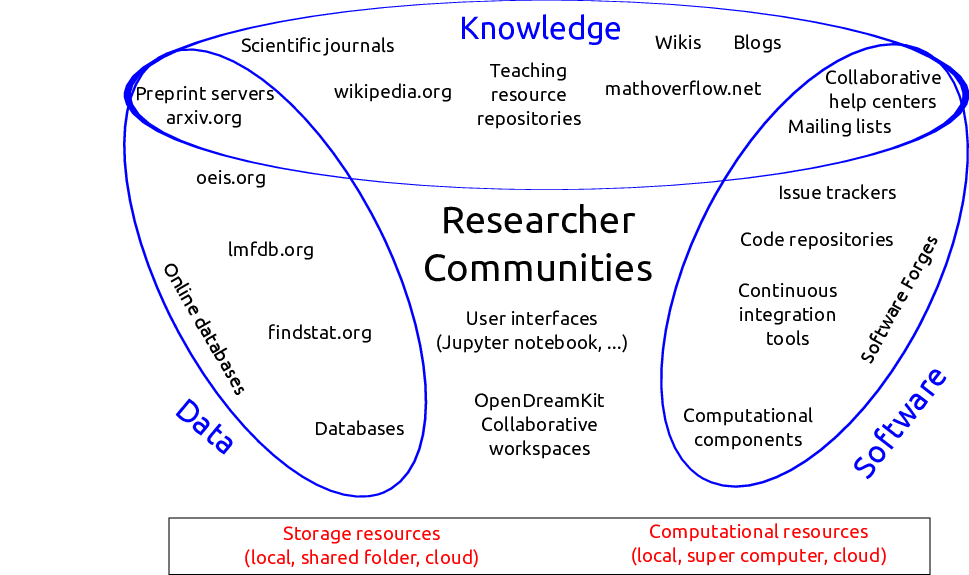
\includegraphics[width=\textwidth]{../../../Proposal/Pictures/TheBigPicture.pdf}
\end{frame}

\begin{frame}{OpenDreamKit (2015-2019)}
  \begin{block}{Open Digital Research Environment Toolkit\\
    for the Advancement of Mathematics}
    \begin{itemize}
    \item H2020 European Research Infrastructures Work
      Programme\\
      Call: Virtual Research Environments
    %\item Submitted: January 2015, Accepted: May 2015
    \item Budget: 7.6 million euros
    \item 15 sites
    \item 50 participants
    \end{itemize}
  \end{block}
\end{frame}
% \begin{block}{50 participants on 15 sites}
%     \begin{itemize}
%     \item France: Paris Sud, Versailles Saint-Quentin, Bordeaux
%       (CNRS), Grenoble, Logilab
%     \item Germany: Kaiserslautern, Bremen
%     \item Great Britain: Oxford, Southampton, Sheffield, St Andrews, Warwick
%     \item Norway: Simula (Oslo)
%     \item Poland: Silesia
%     \item Switzerland: U Zürich
%     \end{itemize}
%   \end{block}
% \end{frame}

\begin{frame}{OpenDreamKit (2015-2019)}
  \begin{block}{Aims}
    \begin{itemize}
    \item Deliver a flexible Virtual Research Environment toolkit
      supporting collaborative work on soft, data, and knowledge
      \pause
    \item Foster the ecosystem of open source software for pure
      mathematics and beyond
    \end{itemize}
  \end{block}

  % \begin{block}{Main tasks}
  %   \begin{itemize}
  %   \item Modularization and interfaces between systems
  %   \item Build, documentation, tests systems
  %   \item Portability, distribution, deployment
  %   \item High Performance
  %   \item Interactive collaborative computing environments
  %   \item Mathematical databases
  %   \item % TODO: expand More semantic in computation, data, ..
  %   \item Research on social aspects of math soft development
  %   \item Community building and training
  %   \end{itemize}
  % \end{block}
\end{frame}

\begin{frame}{Great opportunity, great responsibility}
  We have signed a contract which we need to fulfill
  \pause

  \begin{block}{But more importantly}
    \begin{itemize}
    \item The European taxpayers are entrusting us
    \item Our communities are entrusting us
    \item Our fellow scientists are starving
    \end{itemize}
  \end{block}
  \pause

  \begin{block}{Please, please}
    {\Large Make the most of each euro spent on this project}
    \begin{itemize}
    \item For the aims of this project
    \item For Science
    \end{itemize}
  \end{block}

  \bigskip
  \pause

  \centerline{\Large Listen to your heart and do what's right}
\end{frame}

\end{document}
